\documentclass{beamer}
\usetheme{Madrid}

\usepackage{amsmath, amssymb, amsthm}
\usepackage{graphicx}
\usepackage{listings}
\usepackage[utf8]{inputenc}
\usepackage{hyperref}

\title{6.5.2.4}
\author{EE24BTECH11004 - Ankit Jainar}
\date{\today}

\begin{document}

\frame{\titlepage}

\begin{frame}
\frametitle{Question}
Find the minimum and maximum values of the function:
\[
f(x) = |\sin(4x) + 3|
\]
We need to determine the global extrema (minimum and maximum) of \(f(x)\), which involves both mathematical analysis and numerical computation.
\end{frame}

\begin{frame}
\frametitle{Theoretical Method}
The given function is:
\[
f(x) = |\sin(4x) + 3|.
\]
Let us define \(g(x) = \sin(4x) + 3\), so that \(f(x) = |g(x)|\).  
To find the extrema of \(f(x)\), we first locate the critical points of \(g(x)\), where its derivative is zero.  
\newline

The derivative of \(g(x)\) is:
\[
g'(x) = \frac{d}{dx}[\sin(4x) + 3] = 4\cos(4x).
\]
Setting \(g'(x) = 0\), we find:
\[
\cos(4x) = 0.
\]
The cosine function is zero when:
\[
4x = \frac{\pi}{2} + n\pi \quad \text{where } n \in \mathbb{Z}.
\]
This gives:
\[
x = \frac{\pi}{8} + \frac{n\pi}{4}, \quad n \in \mathbb{Z}.
\]
\end{frame}

\begin{frame}
\frametitle{Theoretical Method}
To analyze the behavior of \(f(x)\), consider the function \(g(x)\) over one period.  
Since \(g(x)\) is periodic, the extrema of \(f(x)\) repeat in each period.

Substituting \(x = \frac{\pi}{8} + \frac{n\pi}{4}\) into \(g(x) = \sin(4x) + 3\), we calculate:
\begin{align*}
g(x)_{\text{max}} &= \sin(4x) + 3 \quad \text{(when \(\sin(4x) = 1\))}, \\
g(x)_{\text{min}} &= \sin(4x) + 3 \quad \text{(when \(\sin(4x) = -1\))}.
\end{align*}
Thus:
\[
f(x)_{\text{max}} = |3 + 1| = 4, \quad f(x)_{\text{min}} = |3 - 1| = 2.
\]
The \textbf{maximum value} of \(f(x)\) is \textbf{4} and the \textbf{minimum value} is \textbf{2}.
\end{frame}

\begin{frame}
\frametitle{Computational Method}
For computational analysis, we numerically determine the extrema using gradient-based optimization techniques.  
\newline

\textbf{Numerical Gradient Computation}
\newline
The gradient of \(f(x)\) is approximated using the central difference formula:
\[
f'(x) \approx \frac{f(x + \delta) - f(x - \delta)}{2\delta},
\]
where \textbf{\(\delta\)} is a \textbf{small step size}. This approach avoids issues with symbolic differentiation and is used in numerical algorithms.
\newline

\textbf{ Finding Minima and Maxima}
\newline
\textbf{Gradient Descent:} For minima, we iteratively move in the direction of the negative gradient:
\[
x_{n+1} = x_n - \mu f'(x_n),
\]
where \textbf{\(\mu\)} is the \textbf{learning rate}.
\end{frame}
\begin{frame}
\textbf{Gradient Ascent:} For maxima, we move in the direction of the positive gradient:
\[
x_{n+1} = x_n + \mu f'(x_n).
\]


Using an initial guess \(x = 0\), step size \(\mu = 0.01\), and convergence threshold \(10^{-5}\), the algorithm converges to the following results:
\begin{align*}
\text{Minimum Value:} & \quad f(x_{\text{min}}) = 2 \quad \text{at } x_{\text{min}} = 0.785, \\
\text{Maximum Value:} & \quad f(x_{\text{max}}) = 4 \quad \text{at } x_{\text{max}} = 0.392.
\end{align*}

\textbf{Comparison:}
The theoretical and computational results match, confirming the accuracy of the method.
\end{frame}

\begin{frame}
\begin{figure}[h!]
   \centering
   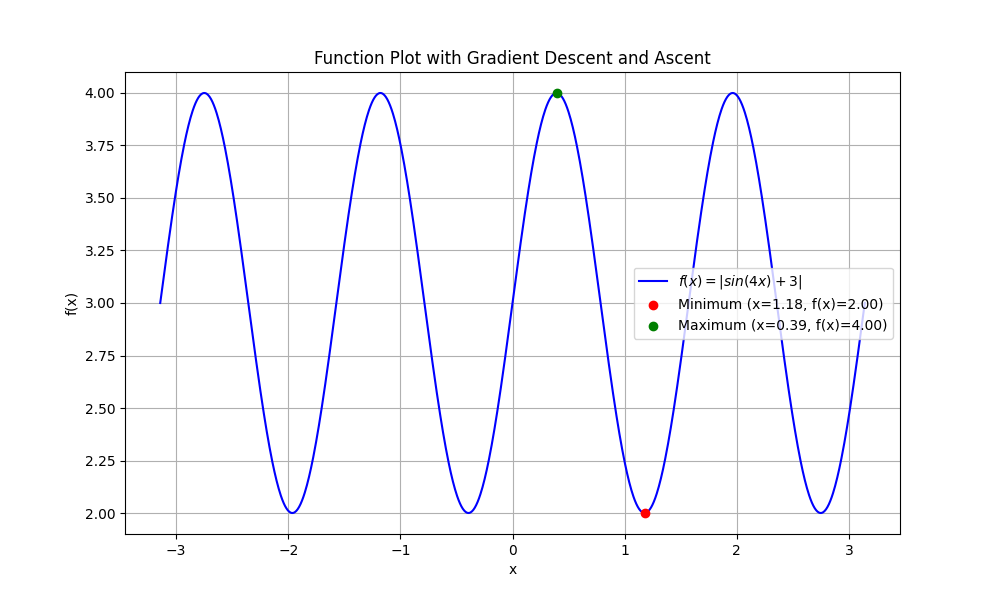
\includegraphics[width=0.7\columnwidth]{figs/fig.png}
   \caption{Graphical Comparison of \(f(x)\) Extrema}
\end{figure}
\end{frame}

\begin{frame}[allowframebreaks]
\frametitle{Conclusion}
The \textbf{maximum value} of \(f(x)\) is 4.\\  
The \textbf{minimum value} of \(f(x)\) is 2.  
\newline

\end{frame}

\end{document}

